\documentclass[conference]{sig-alternate}
%%\documentclass{article} %% hevea
%%\usepackage[utf8]{inputenc} %% hevea

\usepackage[nocompress]{cite}
\usepackage{hyperref}
%% url
\usepackage{url}
%% maths
%%\usepackage[cmex10]{amsmath}
%%\usepackage{amsfonts}
%%\usepackage{amssymb}
%%\usepackage{amsthm}
%% algorithms
\usepackage{algorithm}
\usepackage{algorithmicx}
\usepackage{algpseudocode}
%% images
\usepackage{graphicx}
%% inparaenum
\usepackage{paralist}
%% tables
\usepackage{booktabs}
\usepackage{multirow}
%% figures
\usepackage{subfig}
\usepackage{tikz}
\usetikzlibrary{decorations.pathreplacing,plotmarks,shapes,matrix}
%% transform eps in pdf crossplateform
\usepackage{epstopdf}
\usepackage{epsfig}

\newcommand{\TOFIX}[1]{\textcolor{orange}{#1}}
\newcommand{\TODO}[1]{\textcolor{red}{#1}}

\newcommand{\SCAMP}[0]{\textsc{Scamp}}
\newcommand{\CYCLON}[0]{\textsc{Cyclon}}
\newcommand{\SCAMPLON}[0]{\textsc{Spray}}
%%\newcommand{\SCAMPLONDESCRIPTION}[0]{\footnote{\SCAMPLON{} stands as the contraction of \SCAMP{} and \CYCLON{}.}}
\newcommand{\SCAMPLONDESCRIPTION}[0]{}
\newcommand{\PEERSIM}[0]{\textsc{PeerSim}}

\newcounter{example}
\setcounter{example}{0}
\newcommand{\EXAMPLE}[0]{\stepcounter{example}\the\value{example}}
\newtheorem{definition}{Definition}
\newtheorem{problem}{Problem Statement}
%paralist
\renewcommand*\descriptionlabel[1]{%
\scshape #1}
\renewcommand\paradescriptionlabel[1]{%
\scshape #1}

%%%%%%%%%%%%%%%%%%%%%%%%%%%%%%%%%%%%%%%%%%%%%%%%%%%%%%%%%%%%%%%%%%%%%%%%%%%%%%%
%%%%%%%%%%%%%%%%%%%%%%%%%%%%%%%%%%%%%%%%%%%%%%%%%%%%%%%%%%%%%%%%%%%%%%%%%%%%%%%
%%%%%%%%%%%%%%%%%%%%%%%%%%%%%%%%%%%%%%%%%%%%%%%%%%%%%%%%%%%%%%%%%%%%%%%%%%%%%%%

\begin{document}

\title{Spray: an Adaptive Random Peer Sampling Protocol}

\numberofauthors{5}
\author{
\alignauthor
Brice N{\'e}delec\\
\affaddr{Universit{\'e} de Nantes, LINA}
%\affaddr{2 rue de la Houssini{\`e}re}\\
%\affaddr{Nantes, FRANCE}\\
\email{brice.nedelec{@}univ-nantes.fr}
\alignauthor
Julian Tanke\\
\affaddr{Universit{\'e} de Nantes, LINA}
%\affaddr{2 rue de la Houssini{\`e}re}\\
%\affaddr{Nantes, FRANCE}\\
\email{julian.tanke{@}fu-berlin.de}
\and
\alignauthor
Davide Frey\\
\affaddr{INRIA Bretagne-Atlantique}
%%\affaddr{Campus Universitaire de Beaulieu}\\
%\affaddr{Rennes, FRANCE}\\
\email{davide.frey@irisa.fr}
\alignauthor
Pascal Molli\\
\affaddr{Universit{\'e} de Nantes, LINA}
% \affaddr{2 rue de la Houssini{\`e}re}\\
% \affaddr{Nantes, FRANCE}\\
\email{pascal.molli{@}univ-nantes.fr}
\alignauthor
Achour Mostefaoui\\
\affaddr{Universit{\'e} de Nantes, LINA}
% \affaddr{2 rue de la Houssini{\`e}re}\\
% \affaddr{Nantes, FRANCE}\\
\email{achour.mostefaoui{@}univ-nantes.fr}
}
\date{}

\maketitle

\begin{abstract}

  Peer-sampling protocols are a fundamental mechanism for a number of
  large-scale distributed applications. The recent introduction of
  WebRTC made easy to deploy distributed applications over a network
  of browsers. However, deploying existing peer sampling protocol on
  top of WebRTC raises the issue the adaptivity of peer sampling
  protocols to sudden bursts of popularity over a network that do not
  manage addressing nor routing. \SPRAY is a novel random peer
  sampling protocol designed to dynamically adapt to the network size
  and for efficient connection establishment. Experiments show the
  flexibility of Spray and highlight its efficiency improvement at the
  cost of little overhead. We embeded \SPRAY in a real-time
  decentralized editor running in browsers and ran experiments
  involving up to 600 communicating web browsers. The results
  demonstrate that \SPRAY significantly reduces the network traffic
  according to the number of participants and saves bandwidth.

  % The introduction of WebRTC has opened a new playground for large-scale
  % distributed applications running in web browsers. Peer sampling protocols can
  % be used to maintain connectivity between devices. However, they do not adapt
  % to networks that can grow and shrink.  As a result, traffic can be oversized.
  % In this paper, we address the limitations of current peer sampling approaches
  % by introducing \SPRAY, a novel adaptive peer sampling protocol that maintains
  % local neighborhood tables that logarithmically scale with the total number of
  % network members. Our experiments demonstrate the ability of \SPRAY to adapt to
  % dynamic networks, reducing the number of WebRTC connections needed to maintain
  % browsers connected. To validate our proposal, we built a real-time
  % decentralized editor running in browsers, thus on laptops, tablets and mobile
  % phones. We ran experiments involving up to 600 communicating web browsers. The
  % results demonstrate that \SPRAY significantly reduces the network traffic
  % according to the number of participants and saves bandwidth.
\end{abstract}


% \begin{abstract}
%   The introduction of WebRTC has opened a new playground for large-scale
%   distributed applications consisting of large numbers of directly-communicating
%   web browsers. In this context, gossip-based peer-sampling protocols appear as
%   a particularly promising tool thanks to their inherent ability to build
%   overlay networks that can cope with network dynamics. However, \TODO{the
%     dynamic nature of browser-to-browser communication} combined with the
%   connection establishment procedures that characterize WebRTC make current
%   peer-sampling solutions inefficient or simply unreliable.  In this paper, we
%   address the limitations of current peer-sampling approaches by introducing
%   \SPRAY, a novel peer-sampling protocol designed to avoid the constraints
%   introduced by WebRTC. Unlike most recent peer-sampling approaches, \SPRAY has
%   the ability to adapt its operation to networks that can grow or shrink very
%   rapidly. Our experiments demonstrate the ability of \SPRAY to adapt to dynamic
%   networks and highlight its efficiency improvements with respect to existing
%   protocols. We built a real-time decentralized editor and ran experimentation
%   involving uptill 600 communicating web browsers. Results highlight the
%   benefits brought by \SPRAY's adaptiveness over \TODO{protocols depending} on
%   it.
% \end{abstract}

%%%%\category{C.2.1}{Computer Systems Organization}{Computer-Communication Networks}[Network Architecture and Design]

%%\terms{Network, algorithm, simulation}

%%% Local Variables:
%%% mode: latex
%%% TeX-master: "../paper"
%%% End:



\section{Introduction}

Peer-sampling
protocols~\cite{voulgaris2005cyclon,jelasity2007gossip,tolgyeski2009adaptive}
constitute a fundamental mechanism for a number of large-scale
distributed applications both on the Cloud~\cite{decandia2007dynamo}
and in a peer-to-peer
setting~\cite{Frey09Middleware,voulgaris2005sub,wuhib2009robust}. By
providing each node with a continuously changing partial view of the
network, they make applications resilient to churn~\cite{bertier-d2ht}
and inherently load balancing~\cite{Frey09DSN}. In the context of
video streaming, for example, a peer-sampling protocol makes it
possible to distribute the streaming load over all peers without
requiring the creation and the maintenance of rigid structures like
multiple trees~\cite{Frey09DSN, monod:THESIS}.  

% made browser-to-browser communications easy even
% within complex network environments that involve firewalls, proxies,
% Net Address Translation (NAT) and mobile networks. A simple click on a
% http link in the browser launches a browser-based video-conferencing
% application as in Firefox Hello, a torrent download browser-based application as in
% webtorrent~\cite{webtorrent}, or a decentralized collaborative
% real-time editor as in CRATE~\cite{nedelec2016crate}. Browsers can be
% seen as an application containter and WebRTC as a communication layer
% for distributed applications deployed in browsers. Users start an
% application in their browsers, create a session URL to allow remote
% access and notify other users. Remote participants have just to click
% on this link to deploy the application in their browsers and join the session.

% Many large scale distributed applications relies on gossip-based peer
% sampling protocols such as \CYCLON~\cite{voulgaris2005cyclon} to
% enable information dissemination~\cite{eugster2003lightweight,
%   tolgyeski2009adaptive}, aggregation~\cite{jelasity2004epidemic} or
% network management~\cite{jelasity2009tman, voulgaris2005epidemic}.


The recent introduction of WebRTC~\cite{webrtc} has renewed the
research interest in a variety of applications that require
peer-sampling protocols such as video streaming~\cite{hivejs,smoothcache2},
content-delivery networks~\cite{Zhang:2013:MBC:2465351.2465379}, or
real-time collaborative editors~\cite{nedelec2016crate}. However,
deploying existing peer-sampling protocols on top of WebRTC raises
important technical challenges.
\begin{inparaenum}[(1)]
\item WebRTC does not manage addressing nor routing; this makes
  connection establishement much more costly than on IP networks and
  more likely to fail. 
\item Browsers run on desktops, laptops and mobile phones. This
  requires protocols that reduce resource consumption as much as
  possible.
\item The ability to launch WebRTC sessions through simple HTTP links
  exposes applications to sudden bursts of popularity.  % Suppose
  % massive online lecture platforms allow students to share their
  % notes. Many lectures run in parallel involving various number of
  % students, i.e., from few to thousands. Also, even during the
  % editing
  % session the audience is subject to significant changes in size,
  % going from thousands to hundreds.
\end{inparaenum}
Consider the example of a user who is streaming a video directly from
his mobile phone to some of his friends. The user suddenly witnesses
some dramatic event, and his friends spread the news by twitting the
stream's address. Instantly a huge number of users connect and start
watching the stream on their laptops and phones. The streaming
mechanisms, and the protocols it relies on must be able to adapt to
this sudden burst of popularity, maintaining their quality of service,
while being able to return to their initial configuration when the
popularity burst subsides. 

% Publishing the
%   link to a WebRTC video stream on Twitter can create the buzz and
%   generate massive joins for an unpredictable period of time.

Unfortunately, existing peer-sampling protocols
% Pascal: IMHO not useful here
%, which lie at the bases of several video streaming
%solutions~\cite{Frey09Middleware,Abeni2009,smoothcache20} 
lack this capability. On the one hand, \SCAMP~\cite{ganesh2003peer}
features some form of adaptation but falls short in the context of
WebRTC applications. \SCAMP maintains partial views of size
$\log(n)+k$, $n$ being the number of nodes, and $k$ being a
constant. But its connection establishment process based on random
walks cannot handle the connection failures that often occur in
WebRTC. On the other hand, the most popular approaches like
\CYCLON~\cite{voulgaris2005cyclon} and the whole RPS protocol
family~\cite{jelasity2007gossip} provide application nodes with
fixed-size views of the network based on parameters that have to be
configured at deployment time. This forces developers to oversize
partial views to handle potential bursts, either wasting resources, or
not provisioning for large-enough settings.
%  Unfortunatly, deploying Scamp on
% top of WebRTC fails due to the connection estabilishement failures of
% WebRTC. Another approach is just to oversize partial views and use
% protocol as Cyclon~\cite{voulgaris2005cyclon}. Unfortunatly, this
% approach consumes more ressources and create and renew periodically
% more connections than required. With this approach, small networks
% will end up paying the price of the largest one. It does not also
% provide a way to compute a fan-out that will ensure high delivery rate
% in any situation.
To address this problem, it would in principle be possible to estimate
the real number of network nodes by periodically running an
aggregation protocol~\cite{montresor2004robust}, and by reconfiguring
\CYCLON, or other RPS solutions based on this. However, this aggregation
protocol would have to run quite frequently, resulting in significant
network overhead to anticipate a popularity burst that may never
happen.

% The scientific challenge consists in finding a way to adapt to the
% network size without actually measuring its number of members as
% proposed by Scamp, but running on top of WebRTC.

In this paper, we address the challenge of a dynamically adaptive
peer-sampling, by introducing \SPRAY, a novel random peer-sampling
protocol inspired by both \SCAMP~\cite{ganesh2003peer} and
\CYCLON~\cite{voulgaris2005cyclon}. \SPRAY improves the
state-of-the-art in several ways.
\begin{inparaenum}[(i)]
\item It dynamically adapts the neighborhood of each peer. Thus, the
  number of connections scales logarithmically with the network size.
\item It only uses neighbor-to-neighbor interactions to establish
  connections. Thus, the process takes constant time.
\item It quickly converges to a topology with properties similar to
  those of random graphs. Thus, the network becomes robust to massive
  failures, quickly disseminates information etc.
\item Experiments show the flexibility of \SPRAY and highlight its
  efficiency improvements at the cost of little overhead.
\end{inparaenum}

\SPRAY not only relieves developers from having to foresee the number
of users of their distributed applications, but most importantly it
allows applications to adapt to sudden burst in popularity. We
demonstrate the effectiveness of \SPRAY by simulation in the context
of a large-scale flash-crowd scenario, as well as on a real use case
using \CRATE~\cite{nedelec2016crate}, deployed on Grid'5000. Our
results demonstrate that \SPRAY significantly reduces network traffic
with respect to a standard peer-sampling protocol, while adapting to
the current size of the network.

% , a real-time decentralized editor directly
% running in web browsers, thus on laptops, tablets, or mobile
% phones. We experiment with \CRATE by deploying 600 editors on

The rest of this paper is organized as follows: Section~\ref{sec:relatedwork}
reviews the related work. Section~\ref{sec:problem} states the scientific
problem. Section~\ref{sec:proposal} details the \SPRAY
protocol. Section~\ref{sec:experimentation} presents experimentation results of
\SPRAY and compares them to state-of-the-art. Section~\ref{sec:use-case} details
our experiment with \CRATE, a real-time collaborative editor running in
browsers. We conclude in Section~\ref{sec:conclusion}.

%%% Local Variables:
%%% mode: latex
%%% TeX-master: "../paper"
%%% End:


\section{Related work}
\label{sec:relatedwork}

\begin{figure*}
\centering
\subfloat[Figure A][Access to the network using a signaling server]{
  
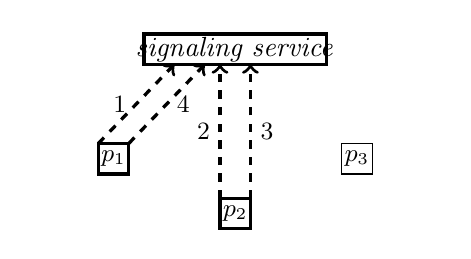
\begin{tikzpicture}[scale=1.1]

\newcommand\X{40pt};
\newcommand\Y{18pt};

\draw( 1.7*\X, 0); %% spacing
\draw(-1.7*\X, 0); %% spacing

\draw[fill=white,very thick](0*\X, 0*\Y) 
node{\emph{signaling service}} +(-30pt,-5pt) rectangle +(30pt,5pt);

\small
\draw[->,dashed, very thick](-5 -1*\X, 5-2*\Y) --
node[anchor=east]{1} (-20pt,-5pt);
\draw[->,dashed, very thick]( 5 -1*\X, 5-2*\Y) --
node[anchor=west]{4} (-10pt,-5pt);

\draw[->,dashed, very thick](-5pt,  5-3*\Y) --
node[anchor=east]{2}(-5pt,-5pt);
\draw[->,dashed, very thick](5pt , 5-3*\Y) --
node[anchor=west]{3} (5pt,-5pt);


\draw[fill=white, very thick]
(-1*\X,-2*\Y) node{$p_1$} +(-5pt,-5pt) rectangle +(5pt,5pt);
\draw[fill=white, very thick]
(0*\X, -3*\Y) node{$p_2$} +(-5pt,-5pt) rectangle +(5pt,5pt);
\draw[fill=white] (1*\X, -2*\Y) node{$p_3$} +(-5pt,-5pt) rectangle +(5pt,5pt);

\end{tikzpicture}

% \begin{tikzpicture}
% \matrix (m) [matrix of math nodes,row sep=4em,column sep=4em] {
% \node(ss)[draw]{signaling}; & \node(p3)[draw]{p3}; \\
% \node(p1)[draw]{p1}; & \node(p2)[draw]{p2}; \\
% };
% \path[->]
%   (p2) edge[dashed] node[fill=white]{1:emit} (ss)
%   (p3) edge[dashed] node[fill=white,bend left]{2:pull} (ss)
%   (p3) edge[dashed, bend right] node[fill=white]{3:accept} (ss)
%   (p2) edge[dashed,bend left] node[fill=white]{4:pull} (ss)
%   (p3) edge[<->,thick] node[fill=white,right]{5:connected} (p2);
% \end{tikzpicture}}
\hspace{20pt}
\subfloat[Figure B][\label{fig:webrtcB}Use the network itself to establish new
connections]{
  
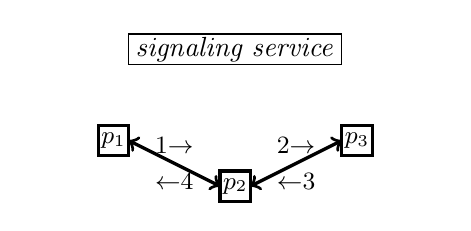
\begin{tikzpicture}[scale=1.1]

\newcommand\X{40pt};
\newcommand\Y{15pt};

\draw(1.7*\X, 0); %% spacing
\draw(-1.7*\X, 0); %% spacing

\draw[fill=white](0*\X, 0*\Y)
node{\emph{signaling service}} +(-35pt,-5pt) rectangle +(35pt,5pt);

\small
\draw[<->, very thick](5-1*\X,-2*\Y)--
node[anchor=south]{1$\rightarrow$}
node[anchor=north]{$\leftarrow$4}(-5pt,-3*\Y);
\draw[<->, very thick](5pt,-3*\Y)--
node[anchor=south]{2$\rightarrow$}
node[anchor=north]{$\leftarrow$3}(-5+1*\X,-2*\Y);

\draw[fill=white, very thick]
(-1*\X,-2*\Y) node{$p_1$} +(-5pt,-5pt) rectangle +(5pt,5pt);
\draw[fill=white, very thick]
(0*\X, -3*\Y) node{$p_2$} +(-5pt,-5pt) rectangle +(5pt,5pt);
\draw[fill=white, very thick]
(1*\X, -2*\Y) node{$p_3$} +(-5pt,-5pt) rectangle +(5pt,5pt);

\end{tikzpicture}

% \begin{tikzpicture}
% \matrix (m) [matrix of math nodes,row sep=4em,column sep=4em] {
% \node(ss)[draw]{signaling}; & \node(p3)[draw]{p3}; \\
% \node(p1)[draw]{p1}; & \node(p2)[draw]{p2}; \\
% };
% \path[->]
%   (p1) edge[dashed,bend left] node[fill=white]{1:emit} (p2)
%   (p2) edge[dashed,bend left] node[fill=white,left]{2:emit/p1} (p3)
%   (p3) edge[dashed,bend left] node[fill=white,right]{3:accept/p1} (p2)
%   (p2) edge[dashed,bend left] node[fill=white]{4:accept} (p1)
%   (p1) edge[<->,thick] (p2)
% %  (p1) edge[<->,thick,bend left] (p3)
%   (p2) edge[<->,thick]  (p3);

% \end{tikzpicture}}
\hspace{20pt}
\subfloat[Figure C][Resulting network overlay]{
  
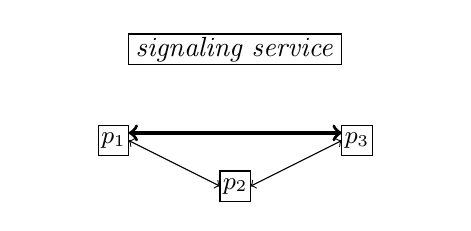
\begin{tikzpicture}[scale=1.1]

\newcommand\X{40pt};
\newcommand\Y{15pt};

\draw(1.7*\X, 0); %% spacing
\draw(-1.7*\X, 0); %% spacing

\draw[fill=white](0*\X, 0*\Y)
node{\emph{signaling service}} +(-35pt,-5pt) rectangle +(35pt,5pt);

\small
\draw[<->](5-1*\X,-2*\Y)--(-5pt,-3*\Y);
\draw[<->](5pt,-3*\Y)--(-5+1*\X,-2*\Y);
\draw[<->, very thick](5 - 1*\X, 2.5 -2*\Y)--(-5+1*\X, 2.5 -2*\Y);

\draw[fill=white]
(-1*\X,-2*\Y) node{$p_1$} +(-5pt,-5pt) rectangle +(5pt,5pt);
\draw[fill=white]
(0*\X, -3*\Y) node{$p_2$} +(-5pt,-5pt) rectangle +(5pt,5pt);
\draw[fill=white]
(1*\X, -2*\Y) node{$p_3$} +(-5pt,-5pt) rectangle +(5pt,5pt);

\end{tikzpicture}


% \begin{tikzpicture}
% \matrix (m) [matrix of math nodes,row sep=4em,column sep=4em] {
% \node(ss)[draw]{signaling}; & \node(p3)[draw]{p3}; \\
% \node(p1)[draw]{p1}; & \node(p2)[draw]{p2}; \\
% };
% \path[->]
%   (p1) edge[<->,thick] (p2)
%   (p1) edge[<->,thick] (p3)
%   (p2) edge[<->,thick]  (p3);
% \end{tikzpicture}}
\caption{\label{fig:webrtc}Creating an overlay network on top of WebRTC.}
\end{figure*}

WebRTC is a protocol that allows real-time communication from
browser-to-browser. It allows establishing a peer-to-peer connection, even with
complex network settings such as firewall, proxies or Net Address Translation
(NAT). Nevertheless, the connection establishment protocol differs from
traditional setting: it requires a round-trip between the browsers to establish
the connection. Figure~\ref{fig:webrtc} depicts the protocol to create a
overlay network on top of WebRTC. Firstly, the joining peer contacts a network
member through a signaling server. Since the connections are repeatedly
established to handle the network dynamicity, the signaling server itself
cannot handle the load of connection requests. On the other hand, each peer can
use the network itself to perform this task. Hence, the network members become
the signaling relays. For instance, Figure~\ref{fig:webrtcB} shows that Peer
$p_1$ uses $p_2$ as relay to reach $p_3$, then $p_3$ answers back using the
same route. Finally, Peer $p_1$ and $p_3$ are connected with a direct
link. \TODO{Explain moar, explain better.}

Random peer sampling protocols~\cite{jelasity2004peer} provide each peer with a
partial view $\mathcal{P}$ of the network membership $\mathcal{N}$. They
populate the partial views with the reference of peers chosen at random among
$\mathcal{N}$ following a uniform distribution using local knowledge
only. Their goal is to converge to an overlay network exposing properties
similar to random graphs~\cite{erdos1959random}. They efficiently provide
connectedness, robustness, messages dissemination etc. A wide variety of
gossip-based protocols use random peer sampling (e.g. topology
management~\cite{voulgaris2005epidemic, jelasity2009tman, dabek2004vivaldi}).

Representatives of random peer sampling protocols~\cite{voulgaris2005cyclon,
  eugster2003lightweight, tolgyeski2009adaptive} use a fixed-size partial view.
Thus, they have to know \emph{a priori} the maximum order of magnitude of the
network size to set their appropriate parameters. These decisions cannot be
safely retracted afterwards. For this reason, the partial views are commonly
oversized compared to the actual network size. While being extremely robust,
they \TODO{generate more traffic}. In the WebRTC context, where the targeted
audience includes small devices such as tablets or mobile phones, the protocols
must be as cheap as possible. One cannot afford to actively maintain $10$
connections when only $3$ are required.

There exists a plethora of network size estimators which would allow re-sizing
the partial views to reflect the network size. These approaches either use
\begin{inparaenum}[(i)]
\item sampling techniques~\cite{mane05network, ganesh2007peer,
    kostoulas2007active} which analyze a network subset and deduce the network
  size using probabilistic functions,
\item sketching techniques~\cite{flajolet2008hyperloglog, baquero2012extrema}
  which use hashing to compress the high amount of data and deduce the network
  size using the collisions,
\item averaging techniques~\cite{jelasity2004epidemic, blasa2011symmetric}
  which use aggregations that converge over exchanges to a value which depends
  of the network size.
\end{inparaenum}
Unfortunately, while they can be very precise in their estimate, they imply a
communication overhead and may have strong assumptions (e.g. random graph
topology).

The sole representative of adaptive-by-design random peer sampling is
\SCAMP{}~\cite{ganesh2001scamp,ganesh2003peer} which stands for SCalable
Membership Protocol. Its interesting property lies in its logarithmically
growing partial view sizes meeting the sharp threshold of connectedness of
random graphs~\cite{erdos1959random}. Nevertheless, \SCAMP{} suffers from other
flaws. In particular, it systematically performs random walks to establish its
connections. In the WebRTC context, each random walk must be traveled back to
finalize the connection establishment. It drastically impacts on the \SCAMP{}
failure probability of establishing a connection. Indeed, let $P_f$ the
probability of either the peer or the link between the latter and the next peer
crashes/disconnects when it holds the traveling message, without any possible
recovery. Let $P_E$ the probability that a connection establishment cannot be
completed. Without three-way handshake, $P_E$ is straightforward:
\begin{equation} P_{E,\,1way}^{Scamp}=1-(1- P_f)^{k+1} \end{equation} where $k$
is the number of hops before the end of the random walk with a minimum of $2$
hops. On the other hand, in the handshaking context, the message must travel
back to its origin in order to be completed. As consequence, when a
subscription travels through a peer or a link, they are not allowed to fail
until the subscription travels back. Thus, we obtain:
\begin{align} P_{E,\,3way}^{Scamp} &=1 - ((1-P_f)^{2(k+1)} (1-P_f)^{2k}
                                     \ldots (1-P_f)^2) \nonumber \\
                                   &=1-(1-P_f)^{k^2+3k+2}
\end{align}
The complexity class of the \SCAMP{} failure rate increases leading to a quick
degenerating number of connections over time. This behaviour endangers the
connectedness of network.

\begin{problem}
  Let $t$ be an arbitrary time frame, let $\mathcal{N}^t$ be the network
  membership at that given time $t$ and let $\mathcal{P}_x^t$ be the partial
  view of peer $p_x \in \mathcal{N}^t$.  A cost-efficient random peer sampling,
  especially when three-way handshaking is involved, should provide the
  following best-case properties:
  \begin{center}
    Partial view size: \hfill
    $\forall p_x \in \mathcal{N}^t,\, |\mathcal{P}_x^t| = \Theta (\ln
    |\mathcal{N}^t|)$
  \end{center}
  \begin{center}
    Connection establishment: \hfill $O(1)$
  \end{center}
  \begin{center}
    Convergence speed: \hfill $\Theta(\exp \, t^{-1})$
  \end{center}
\end{problem}

%%% Local Variables:
%%% mode: latex
%%% TeX-master: "../paper"
%%% End:


\section{Scamplon}
\label{sec:proposal}

Scamplon\footnote{Scamplon stands as the contraction of Scamp and Cyclon.} is a
random peer sampling protocol inspired by both Scamp and Cyclon. It provides
the best of its parents: a logarithmically increasing partial view size
compared to the global network size, and fast convergence to a random graph
using only neighbour-to-neighbour connection establishments. As such, it
constitutes an improvement over state-of-the-art approaches in the common
context of one-way connections. Additionally, it greatly outperforms
state-of-the-art in the three-way handshake connection establishments. The
latter context becomes increasingly important with the apparition of technology
allowing peer-to-peer within modern web browsers. This section details the
Scamplon protocol through intuitions, examples and algorithms.

\begin{algorithm}
  
\small
\algrenewcommand{\algorithmiccomment}[1]{\hskip2em$\rhd$ #1}

\newcommand{\comment}[1]{$\rhd$ #1}


\algblockdefx[initially]{initially}{endInitially}
  [0] {\textbf{INITIALLY:}} 

\algblockdefx[act]{act}{endAct}
  [0] {\textbf{ACTIVE THREAD:}}

\algblockdefx[pas]{pas}{endPas}
  [0] {\textbf{PASSIVE THREAD:}}


\newcommand{\LINEFOR}[2]{%
  \algorithmicfor\ {#1}\ \algorithmicdo\ {#2} %
  }

\newcommand{\LINEIFTHEN}[2]{%
  \algorithmicif\ {#1}\ \algorithmicthen\ {#2} %
  }

\newcommand{\INDSTATE}[1][1]{\State\hspace{\algorithmicindent}}

\begin{algorithmic}[1]
  \Statex
  \initially
    \State $p$ ; \hfill \comment{Identity of the local peer}
    \State $\mathcal{P} \leftarrow [\,]$;
    \hfill \comment{the partial view, sorted by age}
  \endInitially
  
  \act
    \Function{loop}{ } \hfill \comment{Every $\Delta$ time}
    \State $\mathcal{P} \leftarrow incrementAge(\mathcal{P})$;
    \State \textbf{let} $q \leftarrow getOldest(\mathcal{P})$;
    \State \textbf{let} $sample \leftarrow getSample(\mathcal{P}\setminus\left\{q\right\},\, \left \lceil{|\mathcal{P}|\over{2}} \right \rceil) \cup \left\{\langle p,\, 0 \rangle\right\}$;
    \State $sendTo(q,\, sample)$;
    \State \textbf{let} $sample'\leftarrow receiveFrom(q)$;
    \State $\mathcal{P} \leftarrow ((\mathcal{P} \setminus sample) \setminus \left\{ q \right\}) \cup sample'$;  \hfill \comment{update $\mathcal{P}$}
    \EndFunction
  \endAct
  
  \pas
    \Function{onExchange}{$o,\, sample$} \hfill \comment{$o: origin$}
    \State \textbf{let} $sample' \leftarrow getSample(\mathcal{P}\setminus \left\{o\right\} ,\, \left\lceil |\mathcal{P}|\over{2} \right\rceil )  \cup \left\{\langle p,\,0 \rangle\right\}$;
    \State $sendTo(o ,\, sample')$;
    \State $\mathcal{P} \leftarrow ((\mathcal{P} \setminus sample') \setminus \left\{ o \right\}) \cup sample$; \hfill \comment{update $\mathcal{P}$}
    \EndFunction
    \Statex
    \Function{onContact}{$o$} \hfill \comment{$o: origin$}
    \State \LINEFOR{\textbf{each} $q\in\mathcal{P}$}
    {$sendTo(q,\, 'fwdSubs',\, o)$;}
    \State \LINEFOR{$i \leftarrow 0$ \textbf{to} $c$}
    {\INDSTATE $sendTo(\mathcal{P}[\left\lfloor rand()*
        |\mathcal{P}|\right\rfloor],\, 'fwdSubs',\, o)$;}
    \EndFunction
    \Statex
    \Function{onFwdSubs}{$o$} \hfill \comment{$o: origin$}
    \If {$rand() < (1 / (|\mathcal{P}|+1))$}
    \State $\mathcal{P} \leftarrow
    \mathcal{P}\cup \left\{\langle o,\, 0 \rangle\right\}$;
    \Else
    \State $sendTo(\mathcal{P}[\left\lfloor rand()*
      |\mathcal{P}|\right\rfloor],\, 'fwdSubs',\, o)$;
    \EndIf
    \EndFunction
  \endPas
  
\end{algorithmic}

  \caption{\label{algo:scamplon}The Scamplon protocol.}
\end{algorithm}

%%% Local Variables:
%%% mode: latex
%%% TeX-master: "../paper"
%%% End:


\section{Experiments}
\label{sec:experiments}

\subsection{Clustering coefficient}

\subsection{Average path length}

\subsection{Synthesis}

%%% Local Variables:
%%% mode: latex
%%% TeX-master: "../paper"
%%% End:


\section{Conclusion and perspectives}
\label{sec:conclusion}

The introduction of WebRTC has opened a new playground for large-scale
distributed applications consisting of large numbers of directly-communicating
web browsers. Nevertheless, this requires to deploy adaptative peer-sampling
protocols compatible with the WebRTC connection constraints.

In this paper, we described \SPRAY, an adaptative random peer sampling approach
designed to fit the WebRTC constraints.  \SPRAY provides:
\begin{inparaenum}[(i)]
\item logarithmically growing partial views reflecting the global network size,
\item constant time complexity on connection establishments using solely
  neighbor-to-neighbor interactions,
\item an exponentially fast convergence to an overlay network exposing
  properties similar to random graphs.
\end{inparaenum}

% Synthesis of experiments
In experiments, we demonstrated that \SPRAY gently adapts its partial views to
the network size at the price of duplicates. Although, the simulations
supported by theoretical analysis shows that these duplicates stay few in
number and becomes negligible in large networks. Contrarily to \CYCLON, a
representative of fixed-size partial view approaches, \SPRAY automatically
scales to the network size in terms of robustness and efficiency. In
particular, the average shortest path length scales better, the in-degree
evolves with the network size, and it converges faster.  We also demonstrated
that \SPRAY stays robust to massive failures.

% As such, \SPRAY constitutes an improvement over state-of-the-art
% approaches in the traditional context of 1-way connection establishments. In
% addition, the improvement becomes crucial in the 3-way handshake connection
% set-up which is increasingly important since recent technologies (e.g. WebRTC)
% allow peer-to-peer connections between modern web browsers. Random peer
% sampling protocols constitute the ground of many decentralized applications.
% Thus, we expect that decentralized applications (requiring scalable broadcast
% among other) will flourish in the web browsers, while they were previously
% quartered to standalone applications.


Future work includes a Javascript implementation of \SPRAY. An in
browser implementation opens the gate to emulations, and even
real peer-to-peer distributed and decentralized applications.

Future work also includes investigations on topology managers such as
T-Man~\cite{jelasity2009tman} or
Vicinity~\cite{voulgaris2005epidemic}. Indeed, they traditionally rely
on random peer sampling approaches using fixed-size partial
view. Thus, they maintain a fixed-size view of their most closely
related neighbors using a ranking function. With \SPRAY, it is
possible to extend their behavior to use dynamic partial views. If
the view size could adapt to the size of a cluster (if the topology
creates disjoint clusters), it would improve the traffic, robustness,
etc.

%%% Local Variables:
%%% mode: latex
%%% TeX-master: "../paper"
%%% End:


\section*{Acknowledgments}

This work was partially funded by the French ANR project SocioPlug
(ANR-13-INFR-0003), and by the DeSceNt project granted by the Labex CominLabs
excellence laboratory (ANR-10-LABX-07-01).

Experiments presented in this paper were carried out using the Grid'5000
testbed, supported by a scientific interest group hosted by Inria and including
CNRS, RENATER and several Universities as well as other organizations (see
\url{https://www.grid5000.fr}).

%%% Local Variables:
%%% mode: latex
%%% TeX-master: "../paper"
%%% End:


%% Bibliographie
\bibliographystyle{abbrv}
\bibliography{bibliographie}
\clearpage
  
\end{document}

%%% Local Variables:
%%% mode: latex
%%% TeX-master: t
%%% End:
